\documentclass[10pt]{article}
%\usepackage{mathpazo,euler}
\usepackage[utf8]{inputenc}
\usepackage{amsmath}
\usepackage{amsfonts}
\usepackage{amssymb}
\usepackage{amsthm}
\usepackage{mathtools}
\usepackage{graphicx}
\usepackage{enumerate}
\usepackage{ragged2e}
\usepackage{xcolor}
\usepackage{url}
\usepackage{caption}
\usepackage{tikz}
\usepackage{tikz-cd}
%\setlength{\parindent}{0em}
\usepackage[left=2.9cm,right=2.9cm,top=2cm,bottom=2.5cm]{geometry}
\usepackage{pgfplots,tikz,tikz-cd}
\pgfplotsset{compat=1.17}
\author{Ángel Ríos San Nicolás}
\theoremstyle{definition}
\newtheorem{ejer}{Ejercicio}
\newtheorem*{sol}{Solución}
\title{Geometría Discreta y Computación}
\date{Hoja 3--Triangulaciones y subdivisiones\\ 10 de febrero de 2021}
\newcommand{\RR}{\mathbb{R}}
\newcommand{\st}{\operatorname{star}}
\newcommand{\conv}{\operatorname{conv}}
\newcommand{\vol}{\operatorname{vol}}
\newcommand{\aff}{\operatorname{aff}}
\newcommand{\cone}{\operatorname{cone}}
\newcommand{\convaa}{\operatorname{conv}\left(A\setminus\{a_0\}\right)}
\renewcommand{\figurename}{Figura}
\begin{document}
\maketitle

\begin{ejer} {\bf Triangulaciones de un pol\'igono convexo. N\'umeros de Catalan.} 
%(Rescued from sheet 2) 
Para cada $n$, sea $T_n$ el conjunto de todas las triangulaciones de un pol\'igono convexo con $n$ lados. 
%\footnote{Suponemos los $n$ v\'ertices ordenados c\'iclicamente a lo largo del pol\'igono y los denotamos por los n\'umeros $1$ a $n$. Cada triangulaci\'on es una lista de aristas, o de tri\'angulos, dados por sus etiquetas. En particular, el conjunto $T_n$ no depende de qu\'e pol\'igono estemos considerando. Por ejemplo, $T_5$ tiene cinco elementos:
%\[
%\{123,134,145\},
%\{234,245,125\},
%\{345,135,123\},
%\{145,124,24\},
%\{125,235,345\}.
%\]
%}
El objetivo de este ejercicio es demostrar que 
 $T_n$ tiene  $\frac{1}{n-1}\binom{2n-4}{n-2}$ elementos. 
 % For this:
 
\begin{enumerate}[(a)]
\item Comprobar que cada triangulaci\'on del polígono tiene $2n-3$ aristas. % (las $n$ del borde y $n-3$ interiores).
Deduce que el grado medio de los v\'ertices de una triangulaci\'on es 
$4-\frac{6}{n}$.

\item Fijemos un v\'ertice, digamos el $1$. Demostrar que el grado medio *de ese v\'ertice* entre todas las triangulaciones de $T_n$ es tambi\'en
 $4-\frac{6}{n}$. (Pista: esto se sigue de la simetr\'ia y un argumento de doble conteo).
 
\item Consideremos la aplicaci\'on  $\phi: T_{n+1}\to T_{n}$ que ``contrae'' la arista $\{1,n+1\}$, convirtiendo cada triangulaci\'on del 
$(n+1)$-gono en una del $n$-gono.%\footnote{We consider the vertices of the $n$-gon to be labeled from $1$ to $n$ in cyclic order.}

Demostrar que para cada $G\in T_{n}$, el n\'umero de triangulaciones en $\phi^{-1}(G)$ es $\deg_G(1)$ (el grado del v\'ertice $1$ en $G$).

\item Concluir de (b) y (c) que
% the \emph{average} size of $f^{-1}(G)$ is exactly $\frac{4n-6}{n}$.
%\item Deduce that
\[
|T_{n+1}| = \frac{4n-6}{n} |T_n|.
\]
\item Deduce la f\'ormula $|T_n|=\frac{1}{n-1}\binom{2n-4}{n-2}$, por inducci\'on.
\end{enumerate}


{\bf Nota:} los n\'umeros $C_n=\frac{1}{n+1}\binom{2n}{n}$ son los  \emph{n\'umeros de Catalan} que aparecen en muchos contextos.
%\footnote{Ver, por ejemplo, \url{https://www.youtube.com/watch?v=kjn9hFQK9aQ}}
Este ejercicio muestra que $|T_n|$ es el $(n-2)$-\'esimo n\'umero de Catalan.
\end{ejer}
\begin{sol}\leavevmode
\begin{enumerate}[(a)]
    \item Vamos a probar que toda triangulación de un $n$-gono convexo es o un solo triángulo o se puede construir mediante pegado sucesivo de los triángulos que la conforman de manera que en cada paso $3\leq k\leq n$, se construye una triangulación de un $k$-gono a partir de una de un $(k-1)$-gono pegando un triángulo con solo una arista común al $k$-gono, en particular, en cada paso se añaden solo dos aristas, lo que probará el resultado.
    
    Partimos de una triangulación del $n$-gono y tomamos un triángulo cualquiera de la misma. Si $n=3$, hemos terminado porque el polígono original era el propio triángulo.
    
    Si $n\geq 3$, por definición de triangulación, cualquier otro triángulo es disjunto, interseca solo en un vértice, o tiene una arista común. Afirmamos que existe siempre un triángulo con una arista común. Si no fuera así, el resto de triángulos serían disjuntos o existiría uno unido solo por un vértice. En ambos casos el polígono resultante no sería convexo lo que es una contradicción. Por lo tanto, podemos añadir un triángulo unido por una arista. Como el vértice es exterior al polígono, forma un cuadrilátero convexo con dos aristas más. Aplicando el mismo argumento, o hemos completado la triangulación del $n$-gono original y era un cuadrilátero o debe existir un triángulo con una arista común. Podemos repetir este proceso añadiendo triángulos siempre con una arista común de manera que en el último paso construimos una triangulación del $n$-gono original añadiendo un triángulo a una triangulación de un $(n-1)$-gono lo que, en particular, añade exactamente dos aristas.
    
    
    %Lo demostramos por inducción en el número $n$ de lados del polígono. Sabemos que el número de lados es igual al número de vértices. Si $n=3$, el polígono es un triángulo que solo admite la triangulación trivial que es el propio triángulo de $3$ aristas y $2\cdot 3-3=6-3=3$. Suponemos que se cumple para el $(n-1)$, es decir, que toda triangulación de un $(n-1)$-gono convexo tiene $2(n-1)-3$ aristas. Claramente, toda triangulación del $n$-gono se puede construir mediante pegado de los triángulos que la componen. Si empezamos con un triángulo,
    
    Veamos ahora lo que queríamos, que cada triangulación de un $n$-gono tiene $2n-3$ aristas. Lo probamos por inducción. El triángulo tiene una única triangulación con $3$ aristas y $2\cdot 3-3=6-3=3$. Suponemos que se cumple para un $(n-1)$-gono, es decir, que cada triangulación tiene $2(n-1)-3$ aristas y lo probamos para un $n$-gono. Dada una triangulación de un $n$-gono, sabemos que es una triangulación de un $(n-1)$-gono, que, por hipótesis de inducción, tiene $2(n-1)-3$ a la que se añade un triángulo por una arista, lo que solo añade dos aristas más. En total, la triangulación del $n$-gono tiene $2(n-1)-3+2=2n-2-3+2=2n-3$ aristas como queríamos probar.
    
    La suma de los grados de los vértices de una triangulación es el doble del número de aristas con lo que el grado medio de los vértices es 
    \[\frac{1}{n}\sum_{i=1}^n\deg(i)=\frac{2(2n-3)}{n}=4-\frac{6}{n}.\]

\item Por simetría, todo vértice del polígono tiene el mismo grado medio entre todas las triangulaciones y lo denotamos $\partial$. Por definición, se cumple
\[\partial = \frac{1}{|T_n|}\sum_{t\in T_n}\deg_t(1)=\cdots=\frac{1}{|T_n|}\sum_{t\in T_n}\deg_t(n)\]
donde $\deg_t(i)$ denota el grado del vértice $i$ en la triangulación $t\in T_n$.
Sumando todos, tenemos que
\begin{equation}\label{npartial}
    n\partial = \frac{1}{|T_n|}\sum_{i=1}^n\sum_{t\in T_n}\deg_t(i).\tag{$\star$}
\end{equation}
Observamos que en el doble sumatorio estamos sumando los grados de todos los vértices en todas las triangulaciones que es el doble de la suma de todas las aristas en todas las triangulaciones. Por el apartado anterior, cada triangulación tiene $2n-3$ aristas, por lo tanto, en total hay $2(2n-3)|T_n|$ aristas y entonces,
\[n\partial = \frac{1}{|T_n|}2(2n-3)|T_n|=4n-6\longrightarrow \partial=4-\frac{6}{n}.\]

Otra forma de hallar $\partial$ aprovechando el cálculo anterior del grado medio de los vértices de una triangulación es invertir el orden de los sumatorios en \eqref{npartial}. Con eso podemos aplicar que el grado medio de una triangulación es constante independientemente de la triangulación.
\[n\partial = \frac{1}{|T_n|}\sum_{t\in T_n}\sum_{i=1}^n\deg_t(i)=\frac{1}{|T_n|}\sum_{t\in T_n}n\left(4-\frac{6}{n}\right)=\frac{1}{|T_n|}n\left(4-\frac{6}{n}\right)|T_n|=n\left(4-\frac{6}{n}\right).\]
Por lo tanto, el grado medio de un vértice entre todas las triangulaciones es $\partial = 4-\frac{6}{n}$.

\item Sea $G\in T_n$. Consideramos una triangulación en $\phi^{-1}(G)$ y distinguimos dos casos. Si no existe una arista que une el vértice $n+1$ con un vértice $2\leq v\leq n-1$, entonces existe la arista $1(n-1)$ y por tanto el triángulo $\{1n(n+1)\}$. Al aplicar $\phi$ obtenemos la misma triangulación sin ese triángulo y podemos pensar que ahora la arista $n(n+1)$ se ha pegado o está identificada con la arista $1(n-1)$. Si existe una arista que une $n+1$ con un vértice $2\leq v\leq n-1$, consideramos el mínimo $v$ con esa propiedad y distinguimos dos subcasos. Si $v=2$, entonces al aplicar $\phi$ la arista $(n+1)v$ pasa a estar identificada con la arista $12$. Si $v\neq 2$, entonces existe una arista que une $1$ con un vértice $2\leq u\leq v$ y al aplicar $\phi$ la arista $n+1v$ se pega a la arista $1u$. En todas estas transformaciones el resto de aristas se transforma en consecuencia. Las incidentes en $n+1$ pasan a ser incidentes en $1$ y ese vértice de manera que tenemos la triangulación $G$. Las aristas que no son incidentes en $n+1$ no se transforman. Observamos que existe una biyección entre las aristas de $G$ incidentes en $1$ y $\phi^{-1}(G)$ porque la inversa $\phi^{-1}$ consiste en escoger una de las aristas $1u$ y duplicarla de manera que una de las copias pasa a incidir en el vértice $n+1$ y el resto de aristas $1v$ con $v\geq u$ se transforma en consecuencia y hay tantas maneras de hacerlo como aristas incidentes en $1$, es decir, $\deg_G(1)$. Por lo tanto, efectivamente $|\phi^{-1}(G)|=\deg_G(1)$. La siguiente figura es un ejemplo de $\phi^{-1}$ en el caso de una triangulación del pentágono.

\begin{figure}
    \centering
    \begin{tikzcd}
    & 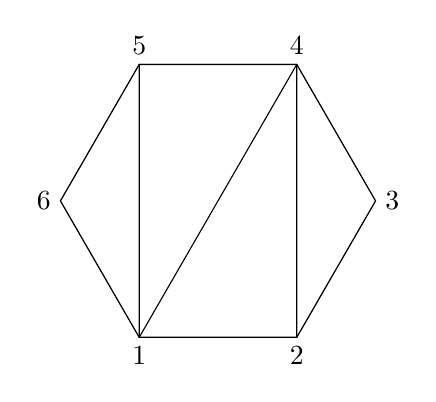
\begin{tikzpicture}[scale=4,cap=round,>=latex]
% Radius of regular polygons
  \newdimen\R
  \R=0.5cm
  \coordinate (center) at (0,0);
 \draw (0:\R)
     \foreach \x in {60,120,...,360} {  -- (\x:\R) }
              -- cycle (300:\R) node[below] {$2$}
              -- cycle (240:\R) node[below] {$1$}
              -- cycle (180:\R) node[left] {$6$}
              -- cycle (120:\R) node[above] {$5$}
              -- cycle (60:\R) node[above] {$4$}
              -- cycle (0:\R) node[right] {$3$};
  \draw (0:\R) \foreach \x in {60,120,...,360} { -- (\x:\R) }
    [fill=white] -- cycle (center);
    \draw (240:\R)--(120:\R)
    (240:\R)--(60:\R)
    (60:\R)--(300:\R);
\end{tikzpicture}\\
    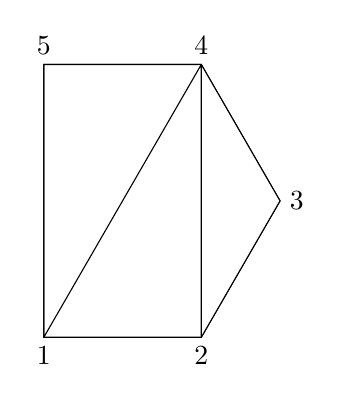
\begin{tikzpicture}[scale=4,cap=round,>=latex]
% Radius of regular polygons
  \newdimen\R
  \R=0.5cm
  \coordinate (center) at (0,0);
 \draw (0:\R)
     \foreach \x in {60,120,240,300,360} {  -- (\x:\R) }
              -- cycle (300:\R) node[below] {$2$}
              -- cycle (240:\R) node[below] {$1$}
              -- cycle (120:\R) node[above] {$5$}
              -- cycle (60:\R) node[above] {$4$}
              -- cycle (0:\R) node[right] {$3$};
  \draw (0:\R) \foreach \x in {60,120,240,300} { -- (\x:\R) }
    [fill=white] -- cycle (center);
    \draw (240:\R)--(120:\R)
    (240:\R)--(60:\R)
    (60:\R)--(300:\R);
\end{tikzpicture}\arrow[ru,mapsfrom,"\phi"]\arrow[r,mapsfrom,"\phi"]\arrow[rd,mapsfrom,"\phi"] & 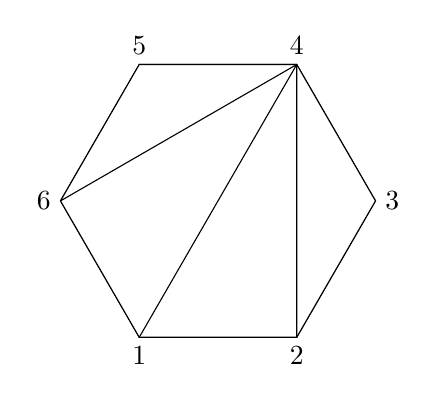
\begin{tikzpicture}[scale=4,cap=round,>=latex]
% Radius of regular polygons
  \newdimen\R
  \R=0.5cm
  \coordinate (center) at (0,0);
 \draw (0:\R)
     \foreach \x in {60,120,...,360} {  -- (\x:\R) }
              -- cycle (300:\R) node[below] {$2$}
              -- cycle (240:\R) node[below] {$1$}
              -- cycle (180:\R) node[left] {$6$}
              -- cycle (120:\R) node[above] {$5$}
              -- cycle (60:\R) node[above] {$4$}
              -- cycle (0:\R) node[right] {$3$};
  \draw (0:\R) \foreach \x in {60,120,...,360} { -- (\x:\R) }
    [fill=white] -- cycle (center);
    \draw (180:\R)--(60:\R)
    (240:\R)--(60:\R)
    (60:\R)--(300:\R);
\end{tikzpicture}\\
    & 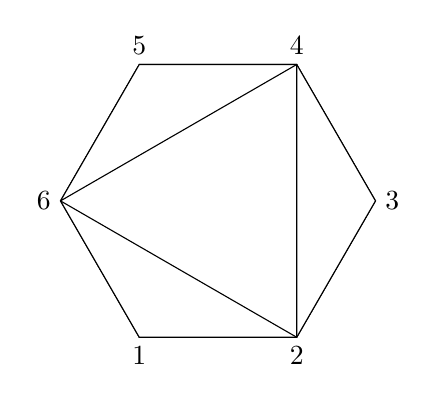
\begin{tikzpicture}[scale=4,cap=round,>=latex]
% Radius of regular polygons
  \newdimen\R
  \R=0.5cm
  \coordinate (center) at (0,0);
 \draw (0:\R)
     \foreach \x in {60,120,...,360} {  -- (\x:\R) }
              -- cycle (300:\R) node[below] {$2$}
              -- cycle (240:\R) node[below] {$1$}
              -- cycle (180:\R) node[left] {$6$}
              -- cycle (120:\R) node[above] {$5$}
              -- cycle (60:\R) node[above] {$4$}
              -- cycle (0:\R) node[right] {$3$};
  \draw (0:\R) \foreach \x in {60,120,...,360} { -- (\x:\R) }
    [fill=white] -- cycle (center);
    \draw (180:\R)--(60:\R)
    (180:\R)--(300:\R)
    (60:\R)--(300:\R);
\end{tikzpicture}
\end{tikzcd}
\caption{Ejemplo de $\phi^{-1}$ para una triangulación del pentágono. Se obtienen tres triangulaciones del hexágono al escoger, de arriba a abajo, la arista $15$, la arista $14$ y la arista $12$ respectivamente.}
\end{figure}

\item El cardinal $|T_{n+1}|$ es la suma de los cardinales de y la aplicación es claramente suprayectiva. Dada una triangulación en $T_n$, se puede construir la triangulación en $T_{n+1}$ en la que solo se añade el triángulo $\{1n(n+1)\}$ de manera que $\Phi$ elimina ese triángulo y la imagen es la triangulación de partida. Por lo tanto,

\[|T_{n+1}|=\sum_{G\in T_n}|\phi^{-1}(G)|=\sum_{G\in T_n}\deg_G(1)=\sum_{G\in T_n}\left(4-\frac{6}{n}\right)=\frac{4n-6}{n}|T_n|.\]

\item Si $n=3$, entonces se cumple claramente porque \[\frac{1}{3-2}\binom{2\cdot 3-4}{3-2}=\frac{1}{2}\binom{2}{1}=1=|T_3|.\] Suponemos que se cumple \[\left|T_n\right|=\frac{1}{n-1}\binom{2n-4}{n-2}\] y queremos probar que \[|T_{n+1}|=\frac{1}{n+1-1}\binom{2(n+1)-4}{n+1-2}=\frac{1}{n}\binom{2n-2}{n-1}.\]
Por el apartado anterior podemos calcular $|T_{n+1}|$ en función de $|T_n|$ y aplicar la hipótesis de inducción.
\[\left|T_{n+1}\right| = \frac{4n-6}{n}\left|T_n\right|
 = \frac{4n-6}{n}\frac{1}{n-1}\binom{2n-4}{n-2}
 = \frac{2(2n-3)(2n-4)!}{n(n-1)(n-2)!(n-2)!}.\]
 Multiplicando numerador y denominador por $(n-1)(2n-2)\neq 0$, tenemos \[\left|T_{n+1}\right|=\frac{2(n-1)(2n-2)(2n-3)(2n-4)!}{n(2n-2)(n-1)(n-2)!(n-1)(n-2)!}=\frac{2(n-1)}{n(2n-2)}\frac{(2n-2)!}{(n-1)!(n-1)!}=\frac{1}{n}\binom{2n-2}{n-1}\]
 como queríamos probar.
\end{enumerate}
\end{sol}

\begin{ejer}{\bf Triangulación ``placing'' o ``pushing''.}
Considérese la siguiente estrategia para triangular una configuración $A$ de puntos en dimensión $d$:
\begin{itemize}
\item Elegir un punto $a_1\in A$ y, recursivamente, suponer que se tiene una triangulación $T_0$ de $A\setminus \{a_1\}$.

\item $T_0$ en particular da una triangulación de cada faceta $F$ de $\conv(A\setminus \{a_1\})$. La denotamos $T_0|_F$. Para cada faceta $F$ que sea visible desde $a$%\footnote{Decimos que una faceta $F$ de un politopo $P$ es visible desde un punto $p$ si el hiperplano que contiene a $F$ separa $a$ del interior de $P$. Esto incluye el caso en que $p\in P$, solo que en ese caso *ninguna* faceta de $P$ es visible desde $P$.}
, añadir a $T_0$ los símplices obtenidos añadiendo $a_1$ a cada símplice de $T_0|_F$.

En el paso recursivo suponemos que se ha usado la misma estrategia, de modo que la triangulación final obtenida depende únicamente de en qué orden se han ido considerando los puntos de $A$.
\end{itemize}

En el paso recursivo suponemos que se ha usado la misma estrategia, de modo que la triangulación final obtenida depende únicamente de en qué orden se han ido considerando los puntos de $A$.

\begin{enumerate}[(a)]
\item Demostrar que esto es una triangulación, o sea, que cubre a $\conv(A)$ y que la intersección de dos símplices cualesquiera es una cara común.

\item Demostrar que la triangulación es regular, obtenida mediante un $w$ en el que se toman $w_i$'s todos positivos, pero cada uno mucho más grande que el siguiente; más explícitamente, si el orden usado es $a_1,\ldots,a_n$ entonces los $w$ en cuestión
\[w_1\gg w_2\gg\cdots \gg w_n>0.\]
\end{enumerate}
\end{ejer}
\begin{sol}\leavevmode
\begin{enumerate}[(a)]
    \item Lo probamos por inducción en el número $n$ de puntos de $A$ menor que la dimensión $d$. 
    
    Si $n=3$, entonces por hipótesis tenemos la triangulación $T_0=\{a_2a_3\}$ que es la única triangulación de dos puntos. Si el punto $a_1$ es interior, no hay nada que probar, no hay facetas visibles desde $a_1$, no hacemos nada y la triangulación queda igual. Si el punto $a_1$ es exterior al segmento $a_2a_3$, distinguimos dos casos. Si $a_1,a_2,a_3$ son colineales, entonces podemos suponer sin pérdida de generalidad que la única faceta de $\conv\left(A\setminus\{a_1\}\right)=a_2a_3$ visible es $F=\{a_2\}$ que posee una única triangulación $T_0|_F=\{a_2\}$ y unimos $a_1$ al símplice y obtenemos la triangulación $T=\{a_1a_3\}$. Si $a_1,a_2,a_3$ son afínmente independientes, entonces las facetas $\{a_2\},\{a_3\}$ de $\conv\left(A\setminus\{a_1\}\right)=a_2a_3$ son visibles desde $a_1$ y uniendo $a_1$ obtenemos la triangulación $T=\{a_1a_2a_3\}$.
    
    Suponemos que se cumple para cardinal $p$, es decir, que si $A=\{a_1,\ldots, a_p\}$ y tenemos una triangulación $T_0$ de $\{a_2,\ldots, a_p\}$, entonces uniendo $a_1$, que suponemos exterior sin pérdida de generalidad, con los símplices de las triangulaciones de todas las facetas $F$ de $\conv\left(A\setminus\{a_1\}\right)$ visibles desde $a_1$ obtenemos una triangulación de $A$, es decir, cubre todo $\conv(A)$ y la intersección de dos símplices es una cara común.
    
    Lo probamos para cardinal $p+1$. Consideramos $A=\{a_0,a_1,\ldots, a_p\}$ y $T_0$ una triangulación de $\{a_2,\ldots,a_p\}$ dada por el procedimiento anterior, cubre $\convaa$ y cumple que la interesección de dos símplice es una cara común. Tenemos $T$ construido uniendo $a_0$, que podemos volver a suponer exterior, con todos los símplices de las triangulaciones $T_0|_F$ de las facetas $F$ de $T$. Tenemos que ver que $T$ es una triangulación.
    \begin{itemize}
        \item Con $T$ cubrimos todo $\conv(A)$. Denotamos por $V$ al conjunto de facetas de $\convaa$ visibles desde $a_0$.
        Observamos que si $F\in V$, entonces para todo símplice $\sigma\in T_0|_F$, que tiene dimensión uno menos, lo que hacemos es añadir el símplice que une $a_0$ con $\sigma$ que cubre $\conv(a_0,\sigma)$. Como lo hacemos en todos los símplices de $F$ cubrimos $\conv(a_0,F)$ con símplices que comparten $a_0$ y, en particular, cubrimos $\cup_{F\in V}\conv(a_0,F)$. La envolvente convexa de los símplices que unen $a_0$ con las facetas visibles desde $a_0$ coincide con $\conv(a_0,V)$ porque $a_0$ se une a las caras visibles. Por lo tanto, se cumple \[\bigcup_{F\in V}\conv(a_0,F)=\conv\left(a_0,\bigcup_{F\in V}F\right).\]
        En particular, cubrimos $\conv(a_0,\bigcup_{F\in V}F)\setminus\left(\convaa\right)$; pero, por hipótesis de inducción, $\convaa$ estaba cubierto por $T_0$ con lo que cubrimos todo $\conv(A)$.
        \item La intersección de dos símplices de $T$ es una cara común. Tomamos $\sigma_1,\sigma_2$ símplices de $T$ con intersección no vacía. Distinguimos tres casos.
        \begin{itemize}
            \item Si $\sigma_1,\sigma_2\in T_0$, la intersección es una cara común por hipótesis de inducción ya que son símplices de la triangulación original.
            \item Si $\sigma_1\in T_0$ y $\sigma_2\in T\setminus T_0$. Necesariamente por construcción $\sigma_1\cap\sigma_2$ es una faceta de $\convaa$ visible desde $a_0$, es $\sigma_1\cap\sigma_2=\conv(a_0,F)$ con $F\in V$ y es claramente una cara común, es una faceta del símplice de unión con $\{a_0\}$. 
            \item Si $\sigma_1,\sigma_2\in T\setminus T_0$, son símplices de unión con $\{a_0\}$. Estos símplices surgen por construcción a partir de facetas de $\convaa$ visibles desde $\{a_0\}$ y hay dos casos. Si las facetas son disjuntas, entonces los símplices de unión solo tienen en común $a_0$ que es una cara común. Si las facetas se cortan, se cortan en una cara común de una dimensión menor. Al unir $a_0$ mediante $\sigma_1$ y $\sigma_2$, esa cara se une de forma convexa por una faceta de ambos símplices que es necesariamente la intersección y una faceta común.
        \end{itemize}
    \end{itemize}
    \item Lo probamos por inducción en el número $n$ de puntos de $A$ menor que la dimensión $d$.
    
    Si $n=3$ y $w:A\longrightarrow\RR$ tal que $w_i=w(a_i)$ con $w_1\gg w_2\gg w_3>0$, entonces la envolvente convexa de $(a_1,w_1),(a_2,w_2),(a_3,w_3)$ es un triángulo o un segmento en $\mathbb{R}^3$ dependiendo de si $A$ es afínmente independiente o los puntos son colineales. Si es un segmento, sus extremos, que podemos suponer que son los levantados de $a_1$ y $a_3$, son inferiores y se proyectan dando la triangulación $\{a_1a_3\}$. Si es un triángulo, sus lados son caras inferiores que se proyectan dando la triangulación $\{a_1a_2,a_1a_3,a_2a_3\}$. Estas dos triangulaciones son las que obteníamos en el caso base de la inducción del apartado anterior.
    
    Suponemos que se cumple para cardinal $p$, es decir, que si $A=\{a_1,\ldots,a_p\}$, la triangulación ``placing'' $T_0$ de $\{a_2,\ldots,a_p\}$ coincide con la que se obtiene proyectando las caras inferiores dadas por un levantamiento $w:A\setminus\{a_1\}\longrightarrow \RR$ tal que \[w_1\gg w_2\gg w_3\gg\cdots\gg w_p>0.\]
    
    Lo probamos para cardinal $p+1$. Si $A=\{a_0,a_1\ldots,a_p\}$, consideramos $w:A\longrightarrow\RR$ un levantamiento tal que 
    \[w_0\gg w_1\gg w_2\gg \cdots\gg w_p>0.\]
    Por hipótesis de inducción, el levantamiento restricción $w|_{A\setminus\{a_0\}}:A\setminus\{a_0\}\longrightarrow \RR$ produce la triangulación ``placing'' $T_0$ de $\{a_1,\ldots,a_p\}$. Esta triangulación se obtiene como restricción de la proyección de las caras inferiores de la envolvente convexa del grafo de $w$. Como $w_0$ es suficientemente mayor que $w_1$, al estar suficientemente por encima que el resto de puntos, el punto levantado $(a_0,w_0)$ solo forma caras simpliciales inferiores con los símplices de los levantados de las triangulaciones de las facetas que son visibles. Al proyectar, estos símplices se transforman en símplices que unen $a_0$ con los símplices de las triangulaciones de las facetas visibles desde $a_0$, por lo que coincide con la triangulación ``placing''. 
\end{enumerate}
\end{sol}

\begin{ejer}{\bf Triangulación ``pulling''.}
Considérese la siguiente estrategia para triangular una configuración $A$ de puntos en dimensión $d$:
\begin{itemize}
\item Elegir un punto $a_1\in A$ y, recursivamente, suponer que para cada faceta $F$ de $\conv(A)$ se tiene una triangulación $T_F$ de $A|_F$
%\footnote{$A|_F$ es la configuración formada por los elementos de $A$ que están en $F$. Es lo que en clase hemos llamado una ``faceta de $A$''}
.

\item Tomar como $T$ el conjunto de símplices obtenido añadiendo $a_1$ a todos los símplices de todas las $T_F$, para las facetas de $F$ que no contienen a $a_1$.
\end{itemize}

En el paso recursivo suponemos que se ha usado la misma estrategia, de modo que la triangulación final obtenida depende únicamente de en qué orden se han ido considerando los puntos de $A$.

\begin{enumerate}[(a)]
\item Demostrar que esto es una triangulación, o sea, que cubre a $\conv(A)$ y que la intersección de dos símplices cualesquiera es una cara común.
\item Demostrar que la triangulación es regular, obtenida mediante un $w$ en el que se toman $w_i$'s todos negativos, pero cada uno de valor absoluto mucho más grande que el siguiente. Es decir:
\[w_1\ll w_2\ll\cdots\ll w_n<0.\]
\end{enumerate}
\end{ejer}
\begin{sol}\leavevmode
\begin{enumerate}[(a)]
    \item Lo probamos por inducción en el número $n$ de puntos de  $A$ menor que la dimensión $d$.
    
    Si $n=3$, tomamos el punto $a_1\in A$ y distinguimos dos casos. Si $a_1,a_2,a_3$ son colineales, entonces independientemente de que $a_1$ sea o no una faceta, no hacemos nada porque si pertence al segmento determinado por $a_2a_3$, unirlo no cambia la triangulación. Si $a_1$ es una faceta, entonces no hacemos nada y uno de $a_2$ o $a_3$ es interno. Si $a_1,a_2,a_3$ son afínmente independientes, entonces tenemos una única triangulación que es el propio triángulo donde $a_1$ es faceta de dos de los símplices $\{a_1a_2\}$ y ya está unido a las dos facetas del tercero $\{a_2a_3\}$ con lo que al aplicar el proceso no cambia nada y ya es una triangulación.
    
    Suponemos que se cumple para cardinal $p$, es decir, que si $A=\{a_1,\ldots,a_p\}$ y tomamos $a_1\in\conv(A)$. Si suponemos que tenemos una triangulación $T|_F$ en cada faceta $F$ de $\conv(A)$, entonces al unir $a_1$ a los símplices de $T|_F$ tales que $a_1\notin F$, obtenemos una triangulación $T$, cubre $\conv(A)$ y la intersección de dos símplices es una cara común.
    
    Lo probamos para cardinal $p+1$. Suponemos que $A=\{a_0,a_1,\ldots,a_p\}$ y que tenemos una triangulación $T|_F$ de cada faceta $F$ de $\conv(A)$. Construimos $T$ uniendo $a_0$ mediante símplices a los símplices de $T|_F$ para cada $F$ faceta de $\conv(A)$ con $a_0\notin F$. Tenemos que probar que $T$ es una triangulación.
    \begin{itemize}
        \item Con $T$ cubrimos todo $\conv(A)$. Denotamos por $N$ al conjunto de facetas de $\conv(A)$ que no contienen a $\{a_0\}$. Consideramos un punto $x\in\conv(A)$. Si $x$ está en una faceta de $\conv(A)$, el punto $x$ está cubierto por $T$ ya que estaba cubierto por $T$ por hipótesis de inducción. Si $x$ no está contenido en ninguna faceta de $\conv(A)$, lo que hemos construido es el convexo $\conv(a_0,\sigma)$ desde $a_0$ para cada $\sigma\in T|_F$ y $F\in N$. Uniendo estos símplices cubrimos los convexos dados por $a_0$ y cada faceta $F\in N$ y también
        \[\bigcup_{\overset{\sigma\in T|_F}{F\in N}}\conv(a_0,\sigma)=\bigcup_{F\in N}\conv(a_0,F).\]
        Pero, como $\conv(A)$ es la envolvente convexa de sus facetas, $x$ está en uno de los conos, no necesariamente en su interior. En cualquier caso son los símplices que hemos añadido y $x$ está cubierto por $T$.
        \item La intersección de dos símplices de $T$ es una cara común. Tomamos $\sigma_1,\sigma_2$ símplices de $T$ con intersección no vacía. Sean $\tau_1,\tau_2$ los respectivos símplices de las facetas $F_1,F_2$ de $\conv(A)$ por los que se une $a_0\notin F_1,F_2$ a mediante $\sigma_1$ y $\sigma_2$. Distinguimos tres casos.
        \begin{itemize}
            \item Si $\tau_1\cap\tau_2=\emptyset$, entonces claramente $\sigma_1\cap\sigma_2=\{a_0\}$ que es una cara común.
            \item Si $\tau_1\cap\tau_2\neq\emptyset$ es una cara común de $\tau_1$ y $\tau_2$, al unir $a_1$ mediante $\sigma_1$ y $\sigma_2$, esa cara se une de forma convexa por una faceta común de ambos símplices que es necesariamente la intersección.
            \end{itemize} 
    \end{itemize}
    \item Lo probamos por inducción en el número $n$ de puntos de $A$ menor que la dimensión $d$.
    
    Si $n=3$ y $w:A\longrightarrow\RR$ tal que $w_i=w(a_i)$ con $w_1\ll w_2\ll w_3<0$, entonces la envolvente convexa de $(a_1,w_1),(a_2,w_2),(a_3,w_3)$ es un triángulo o un segmento en $\mathbb{R}^3$ dependiendo de si $A$ es afínmente independiente o los puntos son colineales. Si es un segmento, sus extremos que podemos suponer que son los levantados de $a_1$ y $a_3$ son inferiores y se proyectan dando la triangulación $\{a_1a_3\}$. Si es un triángulo, sus lados son caras inferiores que se proyectan dando la triangulación $\{a_1a_2,a_1a_3,a_2a_3\}$. Estas dos triangulaciones son las que obteníamos en el caso base de la inducción del apartado anterior. Es exactamente igual que en el ejercicio anterior por la unicidad de las triangulaciones.
    
    Suponemos que se cumple para cardinal $p$, es decir, que si $A=\{a_1,\ldots,a_p\}$ y que la triangulación por ``pulling'' $T_0$ de $\{a_2,\ldots,a_p\}$ coincide con la que se obtiene proyectando las caras inferiores dadas por un levantamiento $w:A\setminus\{a_1\}\longrightarrow \RR$ tal que \[w_1\ll w_2\ll w_3\ll\cdots\ll w_p<0.\]
    
    Lo probamos para cardinal $p+1$. Si $A=\{a_0,a_1\ldots,a_p\}$, consideramos $w:A\longrightarrow\RR$ un levantamiento tal que 
    \[w_0\ll w_1\ll w_2\ll \cdots\ll w_p<0.\]
    Por hipótesis de inducción, el levantamiento restricción $w|_{A\setminus\{a_0\}}:A\setminus\{a_0\}\longrightarrow \RR$ produce la triangulación por ``pulling'' $T_0$ de $\{a_1,\ldots,a_p\}$. Esta triangulación se obtiene como restricción de la proyección de las caras inferiores de la envolvente convexa inferior del grafo de $w$. Como $w_0$ es suficientemente menor que $w_1$,  
    al ser inferior que el resto de puntos, el punto levantado $(a_0,w_0)$ forma caras inferiores simpliciales con todo el resto de símplices levantados de las triangulaciones de las facetas que no lo contienen. Al proyectar, estos símplices se transforman en símplices que unen $a_0$ con los símplices de las triangulaciones de las facetas que no lo contienen, por lo que coincide con la triangulación ``pulling''.

\end{enumerate}

\end{sol}
\clearpage




\end{document}